\documentclass[11pt]{jsk-thesis}

%レイアウト補正
%\usepackage{layout}
%\setlength \voffset {-1.0cm}
%\setlength \hoffset {-1.2cm}
%\setlength \textwidth {17cm}
%\setlength \textheight {24cm}

%パッケージ読み込み
\usepackage[dvipdfmx]{graphicx}
\usepackage[dvipdfmx]{color}
\usepackage{booktabs}
\usepackage{amsmath}
\usepackage{amssymb}
\usepackage{bm}
\usepackage{url}
\usepackage{otf}

%コマンド定義
%表の日付のフォントサイズ変更
\newcommand{\tdate}[1]{\scriptsize{#1}}
%単位"°"
%%\newcommand{\degree}[1]{#1^{\circ}}
%微分演算子関係
\newcommand{\dd}{\mathrm{d}}
\newcommand{\diff}[2]{\frac{\mathrm{d}#1}{\mathrm{d}#2}} %常微分
\newcommand{\diffline}[2]{\mathrm{d}#1/\mathrm{d}#2} %文章中での常微分
\newcommand{\ddiff}[3]{\frac{\mathrm{d}^#1 #2}{\mathrm{d} #3^#1}} %高階常微分
\newcommand{\ddiffline}[3]{\mathrm{d}^#1 #2/\mathrm{d} #2^#1} %文章中での高階常微分
\newcommand{\pdiff}[2]{\frac{\partial #1}{\partial #2}} %偏微分
\newcommand{\pddiff}[3]{\frac{\partial^#1 #2}{\partial #3^#1}} %高階偏微分
\newcommand{\non}[1]{#1^{*}} %無次元化変数

%関数
\newcommand{\erf}{\mathrm{erf}}

%その他
\newcommand{\myfig}[5]{
  \begin{figure}[#1]%
    \begin{center}%
      \includegraphics[width=#2]{#3}%
      \caption{#4}%
      \label{fig:#5}%
    \end{center}%
  \end{figure}%
}
%% \newcommand{\figref}[1]{Fig.\ref{fig:#1}}
%% \newcommand{\seclabel}[1]{\label{sec:#1}}
%% \newcommand{\secref}[1]{第{\bf\ref{sec:#1}}節}

\newcommand{\unit}[1]{\,[\mathrm{#1}]}

%見出し変更
\renewcommand{\figurename}{Fig.}
\renewcommand{\tablename}{Table}



\usepackage{ikuo}%%便利コマンド集.

\usepackage[dvipdfmx]{hyperref}  % 目次や参考文献をリンクにする。
\usepackage{pxjahyper} %% これを入れるとしおりが文字化けしない。out2uniが不要になる。
%% \hypersetup{bookmarksnumbered=true}
\hypersetup{colorlinks=true}
\hypersetup{linkcolor=black}
%% \hypersetup{linkbordercolor=black}
\hypersetup{urlcolor=black}
%% \hypersetup{urlbordercolor=black}
\hypersetup{citecolor=black}
%% \hypersetup{citebordercolor=black}

\usepackage{url} % \url のために必要。パッケージが無い人は探して入れる。
%% \url{http://nile.ulis.ac.jp/~yuka/}のようにして使う。


\newcommand{\FIGDIR}{./fig}        %図を置くディレクトリを指定する
\usepackage{otf}

\date{令和6年度修士論文}
\title{投擲物の重さや身体のパラメータに応じた\\投擲フォーム戦略の研究}
\author{指導教員 水内 郁夫 教授 \\
\ \\
東京農工大学大学院 \\
生物システム応用化学府 生物機能システム科学専攻 \\
\ \\
令和5年度入学\\
23401127\\
{\bf 伊藤 浩平}}

\begin{document}
\setlength{\baselineskip}{20pt}
\maketitle
\tableofcontents

%各章は別ファイルにして以下にinculudeすると良い.
\chapter[序論]%
        {序論}

        \figb{photo.jpg}{width=0.75\hsize}{図1}%

        \fig{fig1.eps}{width=.9\hsize}{何かの図}%

        \section{研究の背景と目的}
        \seclabel{intro}

        投擲動作を行うスポーツは数多く存在するが、野球と砲丸投げのように競技によって投
        擲フォームは異なり、さらに同一競技内であっても個人によって投擲フォームは異なる。
        競技や個人によって投擲フォームが異なる要因として、投擲物や身体といった投擲フォー
        ムに関連するパラメータの違いが挙げられる。
        具体的なパラメータとして、投擲物は重さや大きさ、身体は慣性や各部位のサイズ等がある。
        これまで投擲フォームに関する研究例として、眞田の野球におけるオーバーハンドスローとサイドハンドスロー
        の球速の比較、大室らの野球における足の踏み出し幅による投球速度の比較、黒松らの砲丸投げグライド投法における投擲フォーム改善前後の飛距離の比較などがある。
        投擲フォームは球速や投擲物の飛距離等の、スポーツにおける総合性能に大きな影響を及ぼす。
        また、投擲に関する総合性能の研究例として、蔭山らの野球における年齢による体格や背筋力と投球速度の関係、
        高橋らの野球における肩関節と股関節の可動域・筋力と投球速度の関係、坪井らの砲丸投げにおける
        投射速度・投射角と飛距離の関係などがある。スポーツにおいて総合性能向上は最も重要な要素の一つである。
        これらの研究はある一つの競技に特定した研究である。しかし、さまざまなスポーツに応じた投擲フォームがどのような戦略
        の基で成立しているのかに関する汎用的な理論は確立されていない。
        そこで、本研究ではシミュレーションにおいてさまざまなパラメータに応じた投擲フォームを導出・比較することで、さまざまな投擲フォームの戦略を検討・考察・議論することを目的とする。
        対象となる投擲フォームは、遠投を行うための投擲フォームである。遠投は投射角と手先速度の二つの要素が影響し、それぞれのバランスが求められる。\\
        研究室が散らかっている(\figref{photo.jpg}参照)ので、片付けるロボットが欲
        しい。

        この図(\figref{fig1.eps})はなんだろう?

        \secref{intro}ではほげほげ。

        こういう研究\cite{Ikuo:doctor}もありました。

        ああいう研究\cite{Hondo:JRSJ2011}もありました。

        bibファイルでは、著者名(author=)は、
        「苗字 名前 and 苗字 名前 and 苗字 名前」
        のようにするんですよ\cite{Mizuuchi:RSJ2015-baneoid}。
        間は全部半角スペースですよ。

        \section{従来研究}

        \begin{table}[tb]
          \tablabel{hogehoge}
          \begin{center}
            \caption{試しに作った表}
            \begin{tabular}{l|c|r|r}
              \hline
              項目 & 数値 & コメント & 備考 \\
              \hline
              a & 10.0 & こめんとしがたい & どうすべ?\\
              b & 20.0 & こめんとしがたい & どうすべ?\\
              c & -100.0 & こめんとしがたい & どうすべ?\\
              \hline
            \end{tabular}
          \end{center}
        \end{table}

        \tabref{hogehoge}に、何かの表を示す。

        \section{本論文の構成}

\chapter[強化学習を用いた投擲フォーム導出]{強化学習を用いた投擲フォーム導出}

\section{はじめに}
投擲フォームの導出方法について,本研究では強化学習による最適化手法を採用した.\\
 投擲フォームは競技・個人によって異なる.また,多くの要素が同時に影響する複雑な動作であり,時々刻々と全身の運動連鎖\cite{iwasako}\cite{burkhart}によるダイナミクスが変化するため,明示的な解を求めることは困難である.運動連鎖とは,ある関節の動作が隣接する関節に影響を与え,運動エネルギーを伝達していく運動効果である.強化学習は複雑なモデルや学習プロセスにより最適化までに時間的計算コスト等はかかるが,明示的な解がなく詳細なパラメータ設定が求められる投擲フォーム導出において有効な手段である.

\section{強化学習}
\subsection{強化学習}
強化学習\cite{rl1}\cite{rl2}とは,環境を観測しながらエージェントが試行錯誤することで,獲得する方策を最適化する機械学習の手法である.
方策とは,環境に対してエージェントがどのような行動を選択すべきかを決定する部分である.
強化学習の流れの概略図について,\figref{2.1.jpg}に示す.
\fig{2.1.jpg}{width=1.0\hsize}{Reinforcement Learning mechanism}
エージェントが環境に対して行動を選択し,実行する.環境はその行動に対しエージェントに状態と報酬をフィードバックする.
その後,エージェントは受け取った状態から報酬がより大きくなるような行動を選択する.\\
 この学習を繰り返すことでエージェントは行動を改善し,最適な行動を見つけることができる.
\subsection{強化学習手法}
本研究では,強化学習の手法の1つであるQ学習\cite{watkins}を採用する.Q学習とは,ある状態における,ある行動の価値をQ値と呼ばれる価値関数を用いて表す.
このQ値は短期的な報酬でなく,より報酬の高い状態へと遷移できるかを見据え,行動の長期的な価値を示すものである.\\
 Q学習において,Q値は\equref{Q}で更新する.\\
\begin{eqnarray}
  \equlabel{Q}
  Q(s,a)=(1-\alpha)Q(s,a)+\alpha(r+\gamma \mathrm{max}Q(s',a'))
\end{eqnarray}
\equref{Q}において,$\alpha$は学習率,$\gamma$は割引率であり,範囲はそれぞれ0$\leq$$\alpha$$\leq$1,0$\leq$$\gamma$$\leq$1である.また,$Q(s,a)$は状態が$s$における行動$a$の行動価値関数である.学習率はQ値の更新の大きさを決定するパラメータであり,\equref{Q}におけるQ値の更新量であるTD誤差$\alpha(r+\gamma \mathrm{max}Q(s',a'))$に影響する.学習率が極端に大きすぎるとQ値の更新が過剰となるため学習が発散する.一方,学習率が極端に小さすぎると学習の収束が遅くなり,局所的な最適解にとどまる可能性がある.そのため,Q学習において最適な学習率を設定することが重要である.割引率は将来の価値をどれだけ割り引くのかを決定するパラメータである.割引率が大きいほど長期的な報酬を重要視するため学習の収束に時間を要する.一方,割引率が小さいほど短期的な報酬を重要視するため,最適解に収束しない可能性がある.そのため,学習率と同様に最適な割引率を設定することが重要である.
\subsection{行動選択方法}
本研究では,行動選択方法として$\varepsilon$-greedy法\cite{greedy}を採用した.$\varepsilon$-greedy法とは,探索と活用のトレードオフを管理するための一般的な強化学習の手法である.
$\varepsilon$-greedy法では,$\varepsilon$(0$\leq$$\varepsilon$$\leq$1)の確率で全ての行動からランダムに行動を選択し,1-$\varepsilon$の確率でルールの価値が最も高い行動を選択する.
学習が進んでも$\varepsilon$が大きいと,無駄な探索が増加し学習効率が低下する.そのため,学習が進むにつれて$\varepsilon$を0に近づけることで,より学習したルールの価値に基づいた行動が選択できる.
\subsection{その他}
本論文に登場する強化学習の用語について述べる.\\
\begin{itemize}
  \item エピソード:学習回数.強化学習ではエピソードを重ねるごとにエージェントが行動を改善し,報酬が高くなるように行動していく.
  \item ステップ:1エピソード内でエージェントと環境の相互作用が行われる回数.時間ステップと1エピソード内のステップ数により,1エピソードでエージェントが行う時間を設定することができる.
\end{itemize}

\chapter[剛体1リンクによるリンク速度最適化シミュレーション]{剛体1リンクによる\\リンク速度最適化シミュレーション}

\section{はじめに}
本研究では自作したシミュレータを用いて投擲フォームを導出し,戦略を考察したが,検討に先立ち剛体1リンクモデルでのリンク速度最適化シミュレーションを行い,シミュレータと手法の妥当性について検証した.
\section{動力学モデル}
本章の検証で用いた動力学モデルである剛体1リンクを\figref{3.1.eps}に示す.\\

\fig{3.1.eps}{width=1.0\hsize}{Rigid 1 Link}

ラグランジュの方法\cite{lagrange}を用いて導いた剛体1リンクの運動方程式は,次の通りである.\\
$l_{g}$を重心までの長さとすると,リンクの重心位置$o_{s}$は,

\begin{eqnarray}
  o_{s} = 
              \begin{bmatrix}
              l_{g}\cos\theta\\
              l_{g}\sin\theta
              \end{bmatrix}
\end{eqnarray}

微分すると,

\begin{eqnarray}
  o_{\dot{s}} = 
              \begin{bmatrix}
              -l_{g}\sin\theta \cdot \dot{\theta}\\
              l_{g}\cos\theta \cdot \dot{\theta}
              \end{bmatrix}
\end{eqnarray}

リンク重さを$m$とすると,剛体1リンクの並進運動エネルギー$E_{t}$は,

\begin{eqnarray}
  E_{t} 
  &=&\frac{1}{2}mo_{\dot{s}}{}^T\!o_{\dot{s}} \nonumber \\
  &=&\frac{1}{2}m{l_{g}}^2{\dot{\theta}}^2
\end{eqnarray}

同様に,リンク重心周りの慣性モーメントを$I$とすると,回転運動エネルギー$E_{k}$は,

\begin{eqnarray}
  E_{r} 
  =\frac{1}{2}I{\dot{\theta}}^2
\end{eqnarray}

よって,運動エネルギー$T$は,

\begin{eqnarray}
  T
  &=&E_{t} + E_{r} \nonumber \\
  &=&\frac{1}{2}{\dot{\theta}}^2(m{l_{g}}^2 + I)
\end{eqnarray}

位置エネルギー$T$は,

\begin{eqnarray}
  U
  = mgl_{g}\sin\theta
\end{eqnarray}

ここで,ラグランジュ関数$L$を

\begin{eqnarray}
  L
  =T - U
\end{eqnarray}

とすると,運動方程式は,

\begin{eqnarray}
  \equlabel{3.8}
  \frac{d}{dt}(\frac{\partial L}{\partial \dot{q_{i}}}) - \frac{\partial L}{\partial q_{i}} = f_{i} \quad (i = 1,\cdot\cdot\cdot, n)
\end{eqnarray}

ラグランジュ関数$L$を求め,\equref{3.8}に代入し粘性を考慮すると,運動方程式は,

\begin{eqnarray}
  \equlabel{3.9}
  M\ddot{\theta} + g(\theta) + b(\dot{\theta}) = \tau
\end{eqnarray}

このとき,

\begin{eqnarray}
  M = I + m{l_{g}}^2
\end{eqnarray}

\begin{eqnarray}
  g(\theta) = mgl_{g}\cos\theta
\end{eqnarray}

\begin{eqnarray}
  b(\dot{\theta}) = b\dot{\theta}
\end{eqnarray}

$M$は慣性項,$g(\theta)$は重力項,$b(\dot{\theta})$は粘性項である.

\section{シミュレータの作成}
剛体1リンクを強化学習するためのシミュレータをpythonで実装した.シミュレータでは導出した運動方程式をEuler法\cite{euler}により数値積分し運動学を解くことで,剛体1リンクの角度や角速度を計算した.Euler法は常微分方程式を解く手法の1つである.本章では,\equref{3.13},\equref{3.14}を用いて計算を行った.\\

\begin{eqnarray}
  \equlabel{3.13}
  \theta_{N + 1} = \theta + \dot{\theta} \cdot dt
\end{eqnarray}

\begin{eqnarray}
  \equlabel{3.14}
  \dot{\theta}_{N + 1} = \dot{\theta} + \ddot{\theta} \cdot dt
\end{eqnarray}

Euler法の時間ステップは0.001 s とした.また,各エピソードごとに出力した時系列データを基に,pythonライブラリのmatplotlibによりリンク挙動をアニメーション表示するコードを作成した.
\section{強化学習の設定}
本章の強化学習を行うにあたって,状態,行動,報酬,その他を設定した.
\subsection{状態}
Q学習はQ値をQテーブルと呼ばれる状態と行動で表される表に格納するため,連続値を離散化する必要がある.
状態変数は2つとし,リンクの角度$\theta$と角速度$\dot{\theta}$である.
角度の範囲は$-180$ deg $\leq \theta \leq$ $180$ deg,角速度の範囲は$-2.0$ m/s $\leq \dot{\theta} \leq$ $2.0$ m/sとした.
また,分割数は各状態4分割であり,全ての状態を$4^{2}$=16通りで表すことができる.
\subsection{行動}
行動は,全3通りに設定した.回転ジョイントにかかるトルクの選択肢を$-5.0$ N$\cdot$m,$0$,$+5.0$ N$\cdot$mとし,いずれかを$\epsilon$-greedy法に基づき選択した.
\subsection{報酬}
報酬の設計について,\equref{3.15}に示す.リンクの角速度を報酬とすることで,リンクの角速度を大きくする設定とした.

\begin{eqnarray}
  \equlabel{3.15}
  reward = \dot{\theta}
\end{eqnarray}

\subsection{その他}
本検証において,学習率$\alpha$=0.1,割引率$\gamma$=0.9とした.$\epsilon$は\equref{3.16}であり,エピソードが進むにつれてランダム値を選択する確率を小さくする設定とした.

\begin{eqnarray}
  \equlabel{3.16}
  \epsilon = 0.3 \times 0.99^{(\mathrm{episode} + 1)}
\end{eqnarray}

また,エピソード数を1000,時間ステップ$dt$を0.01,1エピソードあたりのステップ数を3000とし,30 s 間の剛体1リンクのリンク速度最適化シミュレーションを行った.
\section{リンク速度最適化シミュレーション}
\subsection{パラメータの設定}
パラメータの設定について,\tabref{3.1}に示す.$b$は粘性係数である.
\begin{table}[tb]
  \begin{center}
    \caption{Rigid 1 link parameters}
    \tablabel{3.1}
    \begin{tabular}{c|c|c}
      \hline
      Parameters & Unit & Values \\
      \hline
      $m$ & kg & 1.0 or 5.0 or 10.0\\
      $l$ & m & 1.00 \\
      $b$ &  & 0.01 \\
      \hline
    \end{tabular}
  \end{center}
\end{table}
リンクの重さは,1.0 kg,5.0 kg,10.0 kg の3種類とした.
\subsection{結果・考察}
初期条件は,$\theta$ = $-90$ deg ,$\dot{\theta}$ = 0 とした際の,リンク重さに応じたリンク速度最適化シミュレーションを行った結果について述べる.\figref{3.2.eps}はリンク重さ1.0 kg,5.0 kg,10.0 kg の際の報酬の遷移である.また,\figref{3.3.eps}はそれぞれのリンク重さの際の30 s 間のリンク速度の時系列を比較したグラフである.比較の結果,リンク重さによってリンク速度の推移に違いがみられた.特に,$m$=10.0 kg の際にトルクの入力は30秒間 $+ 5$ N$\cdot$m が選択され続けていたが,振動開始直後にややリンク速度が負となる瞬間がある.これはトルク不足の影響が考えられる.リンクを回転させる際,最もトルクが必要な姿勢はリンクを垂直下向きの位置から振り上げるタイミングである.本検証は剛体1リンクで自由度が1のため,他のリンクや関節による干渉を受けずリンクが回転し続けた.リンクや自由度が多くなると,他のリンクや関節による影響でリンク挙動に違いが生じると考えられる.\\
 本検証により,自作したシミュレータと手法の有用性を確認した.次章以降では,腕に見立てた剛体2リンクを動力学モデルとし,投擲フォームの導出・比較,戦略の考察を行う.
\fig{3.2.eps}{width=.70\hsize}{Reward progress in Rigid 1 Link(1.0 kg,5.0 kg,10.0 kg)}
\fig{3.3.eps}{width=1.0\hsize}{Transition in angular velocity of Rigid 1 Link(1.0 kg,5.0 kg,10.0 kg)}


\chapter[2次元剛体2リンクによるパラメータに応じた投擲フォーム戦略の考察]{2次元剛体2リンクによるパラメータに応じた投擲フォーム戦略の考察}

\section{はじめに}
本章では、2次元モデルによる投擲物の重さに応じた投擲フォームの比較により、考察した投擲フォーム戦略について述べる。同様に腕の長さに応じた投擲フォームの比較により、考察した投擲フォーム戦略について述べる。
\section{動力学モデル}
本章の検証で用いた動力学モデルを\figref{4.1.eps}
に示す。人間の腕を肩関節1自由度と肘関節1自由度の計2自由度から構成される2次元剛体2リンクとしてモデル化した。
\fig{4.1.eps}{width=1.0\hsize}{剛体2リンク}
ラグランジュの方法を用いて導いた剛体2リンクの運動方程式は、次の通りである。\\
各リンクの重心位置$o_{s_{1}}$,$o_{s_{1}}$は、

\begin{eqnarray}
  o_{s_{1}} = 
              \begin{bmatrix}
              l_{g1}\cos\theta_{1}\\
              l_{g1}\sin\theta_{1}
              \end{bmatrix}
\end{eqnarray}

\begin{eqnarray}
  o_{s_{2}} = 
              \begin{bmatrix}
              l_{1}\cos\theta_{1} + l_{g2}\cos(\theta_{1} + \theta_{2})\\
              l_{1}\sin\theta_{1} + l_{g2}\sin(\theta_{1} + \theta_{2})
              \end{bmatrix}
\end{eqnarray}

微分すると、

\begin{eqnarray}
  o_{\dot{s}_{1}} = 
              \begin{bmatrix}
              -l_{g1}\sin\theta_{1}\dot{\theta}_{1}\\
              l_{g1}\cos\theta_{1}\dot{\theta}_{1}
              \end{bmatrix}
\end{eqnarray}
\begin{eqnarray}
  o_{\dot{s}_{2}} = 
              \begin{bmatrix}
                -l_{1}\sin\theta_{1}\dot{\theta}_{1} - l_{g2}\sin(\theta_{1} + \theta_{2})(\dot{\theta}_{1} + \dot{\theta}_{2})\\
                l_{1}\cos\theta_{1}\dot{\theta}_{1} + l_{g2}\cos(\theta_{1} + \theta_{2})(\dot{\theta}_{1} + \dot{\theta}_{2})
              \end{bmatrix}
\end{eqnarray}

剛体2リンク全体の並進運動エネルギー$E_{t}$は、各リンクの並進運動エネルギーの合計とすると、

\begin{eqnarray}
  E_{t}
  &=&\frac{1}{2}m_{1}o_{\dot{s}_{1}}{}^T\!o_{\dot{s}_{1}} + \frac{1}{2}m_{2}o_{\dot{s}_{2}}{}^T\!o_{\dot{s}_{2}} \nonumber \\
  &=&\frac{1}{2}m_{1}{l_{g1}}^2{\dot{\theta}_{1}}^2 + \frac{1}{2}m_{2}({{l_{1}}^2}{\dot{\theta}_{1}}^2 + {l_{g2}}^2(\dot{\theta}_{1} + \dot{\theta}_{2})^2 + 2{l_{1}}{l_{g2}}\cos({\dot{\theta}_{1}}^2 + \dot{\theta}_{1}\dot{\theta}_{2}))
\end{eqnarray}

同様に、回転運動エネルギー$E_{r}$は、

\begin{eqnarray}
  E_{r}
  =\frac{1}{2}I_{1}{\dot{\theta}_{1}}^2 + \frac{1}{2}I_{2}(\dot{\theta}_{1} + \dot{\theta}_{2})^2
\end{eqnarray}

全体の運動エネルギー$E_{k}$は、

\begin{eqnarray}
  E_{k}
  =E_{t} + E_{r}
\end{eqnarray}

重力によって生じる位置エネルギーについて、重力方向をg = ${[0 \quad -g]}^T$とすると、上腕リンクの位置エネルギー$E_{p1}$は、

\begin{eqnarray}
  E_{p1}
  =m_{1}gl_{g1}\sin\theta_{1}
\end{eqnarray}

前腕リンクの位置エネルギー$E_{p2}$は、

\begin{eqnarray}
  E_{p1}
  =m_{2}g(l_{1}\sin\theta_{1} + l_{g2}\sin(\theta_{1} + \theta_{2}))
\end{eqnarray}

全体の位置エネルギー$K_{p}$は、

\begin{eqnarray}
  E_{p}
  =E_{p1} + E_{p2}
\end{eqnarray}

ここで、ラグランジュ関数Lを

\begin{eqnarray}
  L
  =E_{k} - E_{p}
\end{eqnarray}

とする。ラグランジュ関数Lを求め、\equref{3.8}に代入すると、$\theta_{1}$についての運動方程式

\begin{eqnarray}
  &&(m_{1}{l_{g1}}^2 + I_{1} + m_{2}({l_{1}}^2 + {l_{g2}}^2)
  + 2l_{1}l_{g2}\cos\theta_{2})\ddot{\theta_{1}} \nonumber \\
  &+& (m_{2}({l_{g2}}^2 + l_{1}l_{g2}\cos\theta_{2}) + I_{2})\ddot{\theta_{2}} \nonumber \\
  &-& m_{2}l_{1}l_{g2}\sin\theta_{2}(2\dot{\theta_{1}}\dot{\theta_{2}} + {\dot{\theta_{2}}}^2)  \nonumber \\
  &+& m_{1}gl_{g1}\cos\theta_{1} + m_{2}g(l_{1}\cos\theta_{1} + l_{g2}\cos(\theta_{1} + \theta_{2})) = \tau_{1}
\end{eqnarray}

$\theta_{2}$についての運動方程式

\begin{eqnarray}
  &&(m_{2}({l_{g2}}^2 + l_{1}l_{g2}\cos\theta_{2}) + I_{2})\ddot{\theta_{1}} + (m_{2}{l_{g2}}^2 + I_{2})\ddot{\theta_{2}} \nonumber \\
  &+& m_{2}l_{1}l_{g2}\sin\theta_{2}{\dot{\theta_{1}}}^2 + m_{2}gl_{g2}\cos(\theta_{1} + \theta_{2}) = \tau_{2}
\end{eqnarray}

を得る。これらを整理すると以下の式となる。

\begin{eqnarray}
  M(\theta)\ddot{\theta} + h(\theta, \dot{\theta}) + g(\theta) + b(\dot{\theta}) = \tau
\end{eqnarray}

このとき、$\theta$=${[\theta_{1} \quad \theta_{2}]}^T$、$\tau$=${[\tau_{1} \quad \tau_{2}]}^T$であり、粘性を考慮すると、

\begin{align}
  M(\theta)= 
            \begin{bmatrix}
              m_{1}{l_{g1}}^2 + I_{1} + m_{2}({l_{1}}^2 + {l_{g2}}^2 + 2l_{2}l{g2}\cos\theta{2}) + I_{2} & m_{2}({l_{g2}}^2 + l_{1}l{g2}\cos\theta_{2}) + I_{2} \\
              m_{2}({l_{g2}}^2 + l_{1}l{g2}\cos\theta_{2}) + I_{2} & m_{2}{l_{g2}}^2 + I_{2}
            \end{bmatrix}
\end{align}

\begin{eqnarray}
  h(\theta, \dot{\theta})=
            \begin{bmatrix}
              -m_{2}l_{1}l_{g2}\sin\theta_{2}(2\dot{\theta_{1}}\dot{\theta_{2}} + {\dot{\theta_{2}}}^2) \\
              m_{2}l_{1}l_{g2}\sin\theta_{2}{\dot{\theta_{1}}}^2
            \end{bmatrix}
\end{eqnarray}

\begin{eqnarray}
  g(\theta)=
            \begin{bmatrix}
              m_{1}gl_{g1}\cos\theta_{1} + m_{2}g(l_{1}\cos\theta_{1} + l_{g2}\cos(\theta_{1} + \theta_{2})) \\
              m_{2}gl_{g2}\cos(\theta_{1} + \theta_{2})
            \end{bmatrix}
\end{eqnarray}

\begin{eqnarray}
  b(\dot{\theta})=
            \begin{bmatrix}
              b_{1}\dot{\theta_{1}} \\
              b_{2}\dot{\theta_{2}}
            \end{bmatrix}
\end{eqnarray}

M($\theta$)は慣性行列、h($\theta$, $\dot{\theta}$)はコリオリ力の項、g($\theta$)は重力項、b($\dot{\theta}$)は粘性項である。
\section{シミュレータの作成}
剛体1リンクを強化学習するためのQ学習シミュレータをpythonで実装した。シミュレータでは導出した運動方程式をEuler法により数値積分し運動学を解くことで、剛体1リンクの角度や角速度を計算する。Euler法は上微分方程式を解く手法の1つである。
\section{強化学習の設定}
\subsection{状態}
状態変数は4つとし、肩関節の角度$\theta_{1}$、角速度$\dot{\theta}_{1}$,肘関節の角度$\theta_{2}$、角速度$\dot{\theta}_{2}$とした。\\
各関節の角度の可動範囲は、-180 deg $\le$ $\theta_{1}$ $\le$ 180 deg、0 $\le$ $\theta_{2}$ $\le$ 150 degとした。
上腕リンク、すなわち肩は本来3自由度でありピッチ軸周りの可動範囲は設定した可動範囲より小さい。しかし、ロール軸、ヨー軸の可動範囲の影響により肩が360度回転しているように見える。よって、本章では2次元でのシミュレーションのため上記の可動範囲とした。
また、各リンクの角速度については、-10.0 m/s $\le$ $\dot{\theta}_{1}$ $\le$ 10.0 m/s、-10.0 m/s $\le$ $\dot{\theta}_{2}$ $\le$ 10.0 m/sとした。
分割数は各状態4分割であり、全ての状態を$4^{4}$=256通りで表すことができる。
\subsection{行動}
行動は、全9通りに設定した。肩関節にかかるトルクを正、0、負の3通り、同様に肘関節にかかるトルクも正、0、負の3通りとした。
これにより、Qテーブルは256$\times$9=2304通りで表すことができる。
\subsection{報酬}
報酬は、リリース時のa$\theta_{v}$と手先速度$v_{2}$の2つの要素から設定した。リリースのa$\theta_{v}$について、で計算した。
\begin{eqnarray}
  \equlabel{2.20}
  \theta_{v}=\theta_{1}+\theta_{2}-90
\end{eqnarray}
\equref{2.20}において、$\theta_{v}$、$\theta_{1}$、$\theta_{2}$の単位はdegである。
また、条件は以下の通りとした。\\
0 $\le$ $\theta_{v}$ $\le$ 45 degのとき、$\frac{\theta_{v}}{45}$\\
45 deg $\le$ $\theta_{v}$ $\le$ 90 degのとき、$\frac{90-\theta_{v}}{45}$\\
90 deg $\le$ $\theta_{v}$ $\le$ 135 degのとき、$\frac{\theta_{v}-90}{45}$\\
135 deg $\le$ $\theta_{v}$ $\le$ 180 degのとき、$\frac{180-\theta_{v}}{45}$\\
$\theta_{v}$ $\le$ 0、180 $\le$ $\theta_{v}$のとき、0\\

この条件により、$\theta_{v}$が45 degまたは135 degのときに報酬最大となる。これは、投擲物の遠投時に最も有効な角度である。
これらの角度からリリース時の角度が離れるにつれて報酬が小さくなっていく。
よって投擲方向は指定せずにより投擲物の飛距離を大きくするためのリリースポイントの報酬を大きくすることができる。\\
手先速度$v_{2}$について、

\begin{eqnarray}
  \equlabel{2.21}
  v_{x2}^{2}=-l_{1}\sin\theta_{1}\cdot\dot{\theta}_{1}-l_2\sin(\theta_{1}+\theta_{2})\cdot(\dot{\theta}_{1}+\dot{\theta}_{2})
\end{eqnarray}

\begin{eqnarray}
  \equlabel{2.22}
  v_{y2}^{2}=-l_{1}\cos\theta_{1}\cdot\dot{\theta}_{1}+l_2\cos(\theta_{1}+\theta_{2})\cdot(\dot{\theta}_{1}+\dot{\theta}_{2})
\end{eqnarray}

\equref{2.21}、\equref{2.22}より、

\begin{eqnarray}
  \equlabel{2.23}
  v_{2}=\sqrt{v_{x2}^{2}+v_{y2}^{2}}
\end{eqnarray}

で求めた。\\

以上の2つの要素より、報酬は$\theta_{v}$$\times$$v_{2}$と設定した。この設定により、遠投を行うための投擲フォームを獲得することができる。
また、リリース時の投射角と手先速度の積とすることで、どちらの要素にも報酬に対する重みを付与することができる。\\
さらに効率的に投擲フォームを獲得するために、罰則として累積消費エネルギーを採用し、\equref{2.26}で計算した。

\begin{eqnarray}
  \equlabel{2.24}
  CE_{1}&=&\int \tau_{1}(t)\cdot\dot{\theta}_{1} dt\\
        &\approx&|\tau_{1}(t)\cdot\dot{\theta}_{1}|\cdot\Delta t
\end{eqnarray}

\begin{eqnarray}
  \equlabel{2.25}
  CE_{2}&=&\int \tau_{2}(t)\cdot\dot{\theta}_{2} dt\\
        &\approx&|\tau_{2}(t)\cdot\dot{\theta}_{2}|\cdot\Delta t
\end{eqnarray}

\equref{2.24}、\equref{2.25}より、

\begin{eqnarray}
  \equlabel{2.26}
  CE=CE_{1}+CE_{2}
\end{eqnarray}

これは、1エピソード内において、ステップごとに消費するエネルギーを計算し、それを加算したものである。
累積消費エネルギーはステップを重ねるごとに大きくなるため、1エピソードの内、最終ステップが最も大きくなる。
シミュレーション上では上腕リンクを回し続けるほど手先速度は大きくなると考えられるが、実際の投擲動作では人間の疲労を考慮する必要がある。
そのため、累積消費エネルギーを罰則として採用することは、疲労を再現することを期待できる。
\subsection{その他}
本章では、\equref{Q}における学習率$\alpha$を0.1、割引率$\gamma$を0.9に設定した。これは将来の報酬を優先的に考慮した学習を期待するためである。
1タイムステップは0.005 sであり、1エピソード内のステップ数は2000、すなわち、10 sとした。エピソード数に関しては、学習が収束するまで制限なく行うものとした。
\section{投擲物の重さに応じた最適投擲フォームの比較}
\subsection{シミュレーション設定}
本検証で用いたパラメータを表\tabref{4.1}に示す。身体のサイズは、身長1.72 m、体重70 kgの人間の各部位のサイズとした。
投擲物は、0.14 kg(野球の硬式球)と7.24 kg(砲丸)とした。
\begin{table}[tb]
  \tablabel{4.1}
  \begin{center}
    \caption{Parameters which are used for 2-link simulation}
    \begin{tabular}{c|c|c}
      \hline
      Parameters & Unit & Values \\
      \hline
      $l_{1}$ & m & 0.32 \\
      $l_{2}$ & m & 0.44 \\
      $l_{f}$ & m & 0.25 \\
      $l_{h}$ & m & 0.19 \\
      $m_{f}$ & kg & 1.12 \\
      $m_{h}$ & kg & 0.42 \\
      $m_{o}$ & kg & 0.14 or 7.24 \\
      $m_{1}$ & kg & 1.96 \\
      $m_{2}$ & kg & 1.68 or 8.78 \\
      $b_{1}$ &  & 0.05 \\
      $b_{2}$ &  & 0.01 \\
      \hline
    \end{tabular}
  \end{center}
\end{table}
重力加速度gを9.8 $m/s^{2}$とする。また、本章では、前腕と手と投擲物の要素を合わせて前腕リンクとしてみなすため、3つの要素を考慮して設定を行った。
前腕の要素として、$l_{f}$を前腕長さ、$m_{f}$を前腕重さ、$l_{h}$を手長さ、$m_{h}$を手重さとした。\\
上腕リンクの重心までの長さ$l_{g1}$、前腕リンクの重心までの長さ$l_{g2}$を、\equref{2.26}、\equref{2.27}により計算した。
\begin{eqnarray}
  \equlabel{2.26}
  l_{g1}=\frac{1}{2}l_{1}
\end{eqnarray}

\begin{eqnarray}
  \equlabel{2.27}
  l_{g2}=\frac{1}{2}m_{f}l_{f}+m_{h}(l_{f}+\frac{1}{2}l_{h}+m_{o}l_{2})/m_{2}
\end{eqnarray}

上腕リンクの慣性モーメント$I_{1}$と前腕リンクの慣性モーメント$I_{2}$を\equref{2.28}、\equref{2.29}により計算した。
\begin{eqnarray}
  \equlabel{2.28}
  I_{1}=\frac{1}{12}m_{1}l_{1}^{2}
\end{eqnarray}
\begin{eqnarray}
  \equlabel{2.29}
  I_{2}=\frac{1}{12}m_{f}l_{f}^{2}+m_{f}l_{g1}^{2}+\frac{1}{12}m_{h}l_{h}^{2}+m_{h}l_{g2}^{2}+m_{o}l_{2}^{2}
\end{eqnarray}

各ステップで与えるトルクについて、肩関節に与えるトルク$\tau_{1}$を\equref{2.30}、肘関節に与えるトルク$\tau_{2}$を\equref{2.31}を基に計算した。

\begin{eqnarray}
  \equlabel{2.30}
  \tau_{1} = \tau_{2} + m_{1}gl_{1}\cos(\theta_{1} + \theta_{2})
\end{eqnarray}

\begin{eqnarray}
  \equlabel{2.31}
  \tau_{2} = (m_{2} + m_{o})gl_{2}\cos(\theta_{1} + \theta_{2})
\end{eqnarray}

腕を360 deg 回転させるとき、重力の影響で$\theta_{1}$、$\theta_{2}$が0から90 deg に振り上げる際に最もトルクが必要である。そのため、$\theta_{1}$ = $\theta_{2}$ = 0の際に各関節にかかるトルクを計算し、その計算結果を基に計算した。また、肘関節の可動範囲は0 $\le$ $\theta_{2}$ $\le$ 150 deg であるが、可動範囲の端である$\theta_{2}$ = 0 または $\theta_{2}$ = 150 degでは、可動範囲内に戻ろうとする力が働く。これを考慮し、可動範囲の端では肘関節が可動範囲内に戻る方向に20 Nm のトルクを加算する設定とした。

野球の硬式球の重さの投擲物と砲丸重さの投擲物のときのそれぞれの\equref{2.26}から\equref{2.31}の計算結果を表\tabref{4.2}に示す。
\begin{table}[tb]
  \tablabel{4.2}
  \begin{center}
    \caption{Calculation Results of $l_{g1}$,$l_{g2}$,$I_{1}$,$I_{2}$}
    \begin{tabular}{c|c|c|c}
      \hline
      Parameters & unit & Values of baseball & Values of cannonball \\
      \hline
      $l_{g1}$ & m & 0.16 & 0.16 \\
      $l_{g2}$ & m & 0.21 & 0.40 \\
      $I_{1}$ & kg $\cdot$ ${m}^2$ & 0.017 & 0.017 \\
      $I_{2}$ & kg $\cdot$ ${m}^2$ & 0.081 & 1.50 \\
      $\tau_{1}$ & Nm & -16, 0, 16 & -47, 0, 47 \\
      $\tau_{2}$ & Nm & -10, 0, 10 & -41, 0, 41 \\
      \hline
    \end{tabular}
  \end{center}
\end{table}

投擲物に応じた投擲フォームの強化学習を行った際の報酬の遷移をに示す。硬式野球の重さの投擲物を投じる投擲フォームは1250エピソード、砲丸の重さの投擲物を投じる投擲フォームは4000エピソードを採用した。
\fig{4.2.eps}{width=1.0\hsize}{報酬の遷移}

\subsection{結果・考察}
$\theta_{1}$、$\theta_{2}$、$\dot{\theta}_{1}$、$\dot{\theta}_{2}$の初期状態はいずれも0としたときの投擲物に応じた投擲フォーム戦略の結果・考察を以下に示す。
\figref{4.2.eps}は強化学習により最適化した、野球の硬式球の重さの投擲物を遠投するための投擲フォーム、\figref{4.2.eps}は強化学習により最適化した、砲丸の重さの投擲物を遠投するための投擲フォームである。投擲フォームは投擲開始からリリースまでとし、リリース時の姿勢は黒の太枠で囲まれたものである。図中の青リンク、橙リンクがそれぞれ上腕リンク、前腕リンクに対応し、赤先が手先の軌跡を示す。2つの投擲フォームの比較により、リリース時の肩関節の角度と軌跡の径の大きさに違いが見られた。野球の硬式球の重さの投擲物を遠投するための投擲フォームは肩関節の角度が約157 deg から屈曲した肘が伸展し、リリース時の上腕の角度は約46 deg であった。一方、砲丸の重さの投擲物を遠投するための投擲フォームは肩関節の角度が約66 deg から屈曲した肘が伸展し、リリース時の上腕の角度は約5 deg であった。\\
\figref{4.1.eps}は投擲開始からリリースまでの肩関節・肘関節の角度、角速度、角加速度、トルクの推移である。\figref{4.2.eps}(左)は野球の硬式球の重さの投擲物を遠投するための投擲フォームの各時系列、\figref{4.2.eps}(右)は野球の硬式球の重さの投擲物を遠投するための投擲フォームの各時系列である。\\
トルクの時系列より、野球の硬式球の重さの投擲物を遠投するための投擲フォームは、肩関節と肘関節の運動連鎖を活かした投擲フォームの傾向が見られた。投擲開始からまず肩関節のトルクによって腕を回転させる。その後、約0.13 s で肩トルクが腕の回転とは逆方向にトルクが生じ、肘のトルクが腕の回転と同方向にトルクが生じリリースを迎える。これは肩関節のエネルギーを肘関節に伝達することでより手先方向のエネルギーを大きくしていると考えられる。また、肩関節と肘関節の角速度の推移より、トルクの入力に運動連鎖の傾向が見られる約0.13 s から肩関節の角速度が減少し肘関節の角速度が増加する。リリース時には肩関節と肘関節の角速度が逆転していることから最後は前腕の振りを如何に大きくするのかが重要であると考えられる。一方、砲丸の重さの投擲物を遠投するための投擲フォームは、肩関節による影響が大きい投擲フォームの傾向が見られた。投擲開始から肩関節のトルクによって腕を回転させる傾向は野球の硬式球の重さの投擲物の際と同様であるが、肩関節のトルクが0となる瞬間が数回生じ、また肘関節のトルクは肘を屈曲させる方向に生じ続けている。これは、肩関節のトルクによる腕の回転はペナルティである累積消費エネルギーへの影響が大きいためそれを抑制するためであると考えられる。また、肘関節のトルクによって肘を屈曲させ続ける傾向にある理由として、モーメントアームを小さくすることで肩の回転に消費するエネルギーを抑制するためであると考えられる。加えて肩関節と肘関節の角速度の推移より、肘関節の角速度が正となるのが遅く、リリースの瞬間も肩関節の角速度が肘関節の角速度より大きい。すなわち、肩関節の影響が野球の硬式球の重さの投擲物を遠投する際よりも大きいと考えられる。

\fig{4.2.eps}{width=.50\hsize}{剛体2リンク}



\section{腕の長さに応じた最適投擲フォームの比較}
\subsection{シミュレーション設定}
本検証で用いたパラメータを表\tabref{4.3}に示す。身体のサイズは、身長1.72 m または 1.90 m 、体重70 kgの人間の各部位のサイズとした。
投擲物は、0.14 kg(野球の硬式球)とした。
\begin{table}[tb]
  \tablabel{4.3}
  \begin{center}
    \caption{Parameters which are used for 2-link simulation}
    \begin{tabular}{c|c|c}
      \hline
      Parameters & Unit & Values \\
      \hline
      $l_{1}$ & m & 0.32 or 0.35 \\
      $l_{2}$ & m & 0.44 or 0.48 \\
      $l_{f}$ & m & 0.25 or 0.28 \\
      $l_{h}$ & m & 0.19 or 0.20 \\
      $m_{f}$ & kg & 1.12 \\
      $m_{h}$ & kg & 0.42 \\
      $m_{o}$ & kg & 0.14 \\
      $m_{1}$ & kg & 1.96 \\
      $m_{2}$ & kg & 1.68 \\
      $b_{1}$ &  & 0.05 \\
      $b_{2}$ &  & 0.01 \\
      \hline
    \end{tabular}
  \end{center}
\end{table}


身長1.72 m の人間に基づいた腕の長さでの投擲のときと身長1.90 m の人間に基づいた腕の長さでの投擲のときのそれぞれの\equref{2.26}から\equref{2.31}の計算結果を表\tabref{4.4}に示す。重力加速度、可動範囲の端での肩関節と肘関節に加算するトルクは、4.4.1節と同様の設定とした。
\begin{table}[tb]
  \tablabel{4.4}
  \begin{center}
    \caption{Calculation Results of $l_{g1}$,$l_{g2}$,$I_{1}$,$I_{2}$}
    \begin{tabular}{l|c|c|r}
      \hline
      Parameters & unit & Values of 1.72 m & Values of 1.90 m \\
      \hline
      $l_{g1}$ & m & 0.16 & 0.18 \\
      $l_{g2}$ & m & 0.21 & 0.23 \\
      $I_{1}$ & kg $\cdot$ ${m}^2$ & 0.017 & 0.018 \\
      $I_{2}$ & kg $\cdot$ ${m}^2$ & 0.020 & 0.099 \\
      $\tau_{1}$ & Nm & -16, 0, 16 & -18, 0, 18 \\
      $\tau_{2}$ & Nm & -10, 0, 10 & -11, 0, 11 \\
      \hline
    \end{tabular}
  \end{center}
\end{table}

投擲物に応じた投擲フォームの強化学習を行った際の報酬の遷移を\figref{4.4.eps}に示す。身長1.72 m の人間に基づいた腕の長さによる投擲フォームは1250エピソード、身長1.90 m の人間に基づいた腕の長さによる投擲フォームは2070エピソードを採用した。
\fig{4.4.eps}{width=1.0\hsize}{報酬の遷移}

\subsection{結果・考察}


\chapter[3次元剛体2リンクによるパラメータに応じた投擲フォームの導出・比較と戦略の考察]{3次元剛体2リンクによるパラメータに応じた投擲フォームの導出・比較と戦略の考察}

\section{はじめに}
前章では2次元モデルでの投擲フォーム戦略の考察を行ったが,3次元に拡張することにより,より人間に近いモデルでの投擲フォーム戦略の考察が可能となると考えられる.そこで本章では,3次元モデルによる投擲物の重さに応じた投擲フォームの比較により,考察した投擲フォーム戦略について述べる.
\section{動力学モデル}
本章で用いた動力学モデルを\figref{5.1.eps}に示す.本章では,\figref{5.2.eps}で示す物理エンジンMuJoCo\cite{mujoco}\cite{mujoco2}に標準搭載されているhumanoidモデル「Unitree G1」\cite{unitreeg1}を改変し,人間の腕を肩関節3自由度と肘関節1自由度の計4自由度から構成される3次元剛体2リンクとしてモデル化した.なお,\figref{5.1.eps}において,肩関節から肘関節までを上腕リンク,肘関節から手先までを前腕リンクとし,手首や指の自由度は0とした.また,体幹リンクも自由度0とし,世界座標に固定した.

\section{シミュレータの作成}
3次元剛体2リンクを強化学習するためのQ学習シミュレータをpythonで実装した.運動方程式は,MuJoCoで内部的に解いた.runge-kutta法により数値積分し運動学を解くことで,3次元剛体2リンクの角度や角速度を計算する.
\section{可動範囲}
本章における可動範囲を\tabref{5.1}に示す.それぞれの可動範囲は,各自由度のそれぞれの静的な可動範囲\cite{range}に基づいて設定した.\figref{5.6.eps}が各自由度0 deg の際の各平面からの姿勢であり,MuJoCoにおける回転方向は右ねじの法則に基づいて定義されている.各軸の回転方向は次の通りである.

肩関節ピッチ軸周りの回転:肩関節の伸展方向が正,屈曲方向が負
肩関節ロール軸周りの回転:肩関節の内転方向が正,外転方向が負
肩関節ヨー軸周りの回転:肩関節の内旋方向が正,外旋方向が負
肘関節周りの回転:肩関節の伸展方向が正,屈曲方向が負

\fig{5.6.eps}{width=1.0\hsize}{Model viewed from each plane}

\begin{table}[tb]
  \tablabel{5.1}
  \begin{center}
    \caption{Range of motion: shoulder 3 degrees of freedom, elbow 1 degree of freedom}

    \begin{tabular}{c|c|c|c}
      \hline
      Freedom & Unit & Min Range & Max Range \\
      \hline
      Shoulder pitch & deg & -135 & 45 \\
      Shoulder roll & deg & -135 & -35 \\
      Shoulder yaw & deg & -150 & 180 \\
      elbow pitch & deg & -20 & 90 \\
      \hline
    \end{tabular}
  \end{center}
\end{table}

\tabref{5.1}の可動範囲は各自由度ごとに見ると人間が可能な姿勢である.しかし人間の各関節は互いに干渉するため,組み合わせ次第では人間が不可能な姿勢となる.よって,肩関節ピッチ軸周り,ロール軸周り,ヨー軸周り,肘関節周りの順に,可動範囲を人間が可能な姿勢に収まるように設定した.\\
まず,肩関節ピッチ軸周りの可動範囲に基づいた肩関節ロール軸周りの可動範囲について確認したところ,全ての可動範囲で人間が可能な姿勢であったためそのまま可動範囲として採用した.次に肩関節ピッチ軸周りとロール軸周りに基づいた可動範囲について確認したところ,組み合わせ次第で人間が不可能な姿勢を取ることを確認した.そこで,スプライン補間\cite{spline}を用いて肩関節ピッチ軸周りとロール軸周りの角度によって可動範囲が変動するように設定した.最後に肩関節に基づいた肘関節について確認したところ,全ての可動範囲で人間が可能な姿勢であったため,そのまま可動範囲として設定した.以上の設定により,全ての関節角度の組み合わせで人間が可能な姿勢を取ることができる.なお,計算精度上,数 deg 可動範囲外の角度を取ることがあるが,異常姿勢ではないため問題ないとした.

\fig{5.1.eps}{width=0.8\hsize}{3D rigid body 2 links}
\fig{5.2.eps}{width=0.8\hsize}{Unitree G1}

\section{強化学習の設定}
\subsection{状態}
状態変数は8つとし,肩関節ピッチ軸まわりの角度$\theta_{p}$,角速度$\dot{\theta}_{p}$,肩関節ロール軸まわりの角度$\theta_{r}$,角速度$\dot{\theta}_{r}$,肩関節ヨー軸まわりの角度$\theta_{y}$,角速度$\dot{\theta}_{y}$,肘関節の角度$\theta_{e}$,角速度$\dot{\theta}_{e}$とした.\\
各関節の角度については,5.4章の通りである.
また,各関節の角速度については,-10.0 m/s $\le$ $\dot{\theta}_{1}$ $\le$ 10.0 m/s,-10.0 m/s $\le$ $\dot{\theta}_{2}$ $\le$ 10.0 m/sとした.
分割数は各角度が5分割,各角速度が2分割であり,全ての状態を$5^{4}\times 2^{4}$=10000通りで表すことができる.
\subsection{行動}
行動は,全625通りに設定した.肩関節にかかるトルクを正2通り,0,負2通りの計5通り,同様に肘関節にかかるトルクも正2通り,0,負2通りの計5通りとした.
これにより,Qテーブルは10000$\times$625=6250000通りで表すことができる.
\subsection{報酬}
本章では,投擲物の飛距離を報酬とした.投擲物のモデル化は行っていないため,投射中の投擲物に生じる空気抵抗等は考慮しないものとする.\\
飛距離の計算にあたり,ピッチ,ロール,ヨーの3方向成分の手先速度をMuJoCoより取得し,それぞれ$v_{p}$,$v_{r}$,$v_{y}$とした.手先速度成分の合成は,

\begin{eqnarray}
  \equlabel{5.1}
  v_{syn} = \sqrt{v_{p}^{2} + v_{r}^{2} + v_{y}^{2}}
\end{eqnarray}

\begin{eqnarray}
  \equlabel{5.2}
  v_{pr} = \sqrt{v_{p}^{2} + v_{r}^{2}}
\end{eqnarray}

であり,\equref{5.1},\equref{5.2}より投射角$\theta_{v}$は,

\begin{eqnarray}
  \equlabel{5.3}
  \theta_{v} = \arctan2(\frac{v_{y}}{v_{pr}})
\end{eqnarray}

各ステップ時のヨー軸成分の座標$h_{y}$を手先高さとする.しかし,この座標は肩関節を原点とした時の値であり,本来の手先高さは地面から肩関節までの高さを考慮する必要がある.よって,身長を$L$としたときの手先高さ$h$は,

\begin{eqnarray}
  \equlabel{5.4}
  h = 0.818L + h_{y}
\end{eqnarray}

リリース時の手先高さを考慮した投射時間$t$は,

\begin{eqnarray}
  \equlabel{5.5}
  t = \frac{v_{syn}\sin\theta_{v} + \sqrt{{v_{syn}}^2\sin^2\theta_{syn} + 2gh}}{g}
\end{eqnarray}


以上より,飛距離$D$は\equref{5.1},\equref{5.3},\equref{5.5}を用いて,

\begin{eqnarray}
  \equlabel{5.6}
  D = v_{syn} \cdot \cos\theta_{v} \cdot t
\end{eqnarray}

この報酬により,より直接的に遠投を行うための投擲フォームを導出することができる.また,2次元のときと同様に,罰則として累積消費エネルギーを採用し,\equref{5.11}で計算した.

\begin{eqnarray}
  \equlabel{5.7}
  CE_{p}&=&\int \tau_{p}(t)\cdot\dot{\theta}_{p} dt\\
        &\approx&|\tau_{p}(t)\cdot\dot{\theta}_{p}|\cdot\Delta t
\end{eqnarray}

\begin{eqnarray}
  \equlabel{5.8}
  CE_{r}&=&\int \tau_{r}(t)\cdot\dot{\theta}_{r} dt\\
        &\approx&|\tau_{r}(t)\cdot\dot{\theta}_{r}|\cdot\Delta t
\end{eqnarray}

\begin{eqnarray}
  \equlabel{5.9}
  CE_{y}&=&\int \tau_{y}(t)\cdot\dot{\theta}_{y} dt\\
        &\approx&|\tau_{y}(t)\cdot\dot{\theta}_{y}|\cdot\Delta t
\end{eqnarray}

$\tau_{p},\tau_{r},\tau_{y}$はそれぞれ肩関節ピッチ軸まわり,ロール軸まわり,ヨー軸まわりに与えるトルクである.また,$CE_{p},CE_{r},CE_{y}$はそれぞれ肩関節ピッチ軸まわり,ロール軸まわり,ヨー軸まわりの累積消費エネルギーであり,肩関節の累積消費エネルギーの合計は,

\begin{eqnarray}
  \equlabel{5.10}
  CE_{s} = CE_{p} + CE_{r} + CE_{y}
\end{eqnarray}

肘関節の累積消費エネルギーは,

\begin{eqnarray}
  \equlabel{5.11}
  CE_{e}&=&\int \tau_{e}(t)\cdot\dot{\theta}_{e} dt\\
        &\approx&|\tau_{e}(t)\cdot\dot{\theta}_{e}|\cdot\Delta t
\end{eqnarray}

$\tau_{e}$は肘関節に与えるトルクである.よって,全体の累積消費エネルギーは,

\begin{eqnarray}
  \equlabel{5.12}
  CE = CE_{s} + CE_{e}
\end{eqnarray}

以上より,報酬の設計は,
\begin{eqnarray}
  \equlabel{5.13}
  Reward = D - CE
\end{eqnarray}

\subsection{その他}
本章では,\equref{Q}における学習率$\alpha$を0.1,割引率$\gamma$を0.9に設定した.これは将来の報酬を優先的に考慮した学習を期待するためである.
1タイムステップは0.001 sであり,1エピソード内のステップ数は3000,すなわち,3 sとした.エピソード数に関しては,10000エピソードの中で最も報酬が高いエピソードを採用した.

\section{投擲物の重さに応じた最適投擲フォームの比較}
\subsection{シミュレーション設定}
本検証で用いたパラメータを\tabref{5.3}に示す.身体のサイズは,身長1.72 m,体重70 kgの人間の各部位のサイズとした.
投擲物は,野球の硬式球と砲丸の重さを参考に,0.14 kg と7.24 kg とした.
\begin{table}[tb]
  \tablabel{5.3}
  \begin{center}
    \caption{Parameters which are used for 2link-4DOF simulation}

    \begin{tabular}{c|c|c}
      \hline
      Parameters & Unit & Values \\
      \hline
      $l_{1}$ & m & 0.32 \\
      $l_{2}$ & m & 0.44 \\
      $l_{f}$ & m & 0.25 \\
      $l_{h}$ & m & 0.19 \\
      $m_{f}$ & kg & 1.12 \\
      $m_{h}$ & kg & 0.42 \\
      $m_{o}$ & kg & 0.14 or 7.24 \\
      $m_{1}$ & kg & 1.96 \\
      $m_{2}$ & kg & 1.68 or 8.78 \\
      \hline
    \end{tabular}
  \end{center}
\end{table}
重力加速度gを9.8 $m/s^{2}$とする.また,前章と同様に,前腕と手と投擲物の要素を合わせて前腕リンクとしてみなすため,3つの要素を考慮して設定を行った.
前腕の要素として,$l_{f}$を前腕長さ,$m_{f}$を前腕重さ,$l_{h}$を手長さ,$m_{h}$を手重さとした.\\

次に,野球の硬式球の重さの投擲物と砲丸重さの投擲物のときのそれぞれの上腕・前腕リンクの重心までの長さ,上腕・前腕リンクの慣性モーメント,肩関節の3軸まわり・肘関節に与えるトルク,肩関節の3軸まわり・肘関節の粘性について,表\tabref{5.4}に示す.各リンクの重心までの長さと慣性モーメントについての計算は,\equref{2.26}から\equref{2.31}を基に行った.各関節に与えるトルクについて,肩関節ピッチ軸とロール軸,肘関節はそれぞれ5種類のトルクから選択される.一方,肩関節ヨー軸周りのトルクについては,スプライン補間によって設定した可動範囲に基づき,可動範囲内にトルクが収まるように与えるトルクも補完する設定とした.

\begin{table}[tb]
  \tablabel{5.4}
  \begin{center}
    \caption{Calculation Results of $l_{g}$,$I$,$\tau$,$b$}

    \begin{tabular}{c|c|c|c}
      \hline
      Parameters & unit & Values of baseball & Values of cannonball \\
      \hline
      $l_{g1}$ & m & 0.16 & 0.16 \\
      $l_{g2}$ & m & 0.21 & 0.40 \\
      $I_{1}$ & kg $\cdot$ $\mathrm{m}^2$ & 0.017 & 0.017 \\
      $I_{2}$ & kg $\cdot$ $\mathrm{m}^2$ & 0.15 & 1.59 \\
      $\tau_{p}$ & Nm & -40, -20, 0, +20, +40 & -40, -20, 0, +20, +40 \\
      $\tau_{y}$ & Nm & -40, -20, 0, +20, +40 & -40, -20, 0, +20, +40 \\
      $\tau_{e}$ & Nm & -30, -15, 0, +15, +30 & -30, -15, 0, +15, +30 \\
      $b_{p}$ &  & 1.0 & 1.0\\
      $b_{r}$ &  & 0.8 & 0.8\\
      $b_{y}$ &  & 0.5 & 0.5\\
      $b_{e}$ &  & 0.2 & 0.2\\
      \hline
    \end{tabular}
  \end{center}
\end{table}

以上の設定をふまえ,投擲物に応じた投擲フォームの強化学習を行った際の報酬の遷移を\figref{5.9.eps}に示す.重さ0.14 kg の投擲物を遠投する投擲フォームは2983エピソード,重さ7.24 kg の投擲物を遠投する投擲フォームは9140エピソードを採用した.

\fig{5.9.eps}{width=1.0\hsize}{Reward progress(left: 0.14 kg thrown object,right: 7.24 kg thrown object)}

\subsection{結果・考察}
初期状態について,$\theta_{p}$,$\theta_{r}$,$\theta_{y}$,$\theta_{e}$,$\dot{\theta}_{p}$はランダム値,$\dot{\theta}_{r}$,$\dot{\theta}_{y}$,$\dot{\theta}_{e}$は0とした.これにより,最も報酬が高くなる時の初期姿勢を導出することができる.投擲物に応じた遠投をするための投擲フォーム戦略の結果・考察を以下に示す.
\figref{5.11.eps},\figref{5.12.eps}は強化学習により最適化した,重さ0.14 kg の投擲物を遠投するための投擲フォームである.\figref{5.11.eps}はピッチ軸に垂直な面から見た投擲フォーム,\figref{5.12.eps}はロール軸に垂直な面から見た投擲フォームである.また,\figref{5.13.eps},\figref{5.14.eps}は強化学習により最適化した,重さ7.24 kg の投擲物を遠投するための投擲フォームである.\figref{5.13.eps}はピッチ軸に垂直な面から見た投擲フォーム,\figref{5.14.eps}はロール軸に垂直な面から見た投擲フォームである.リリース瞬間は,1エピソードの中で最も報酬が高いステップとした.投擲フォームは投擲開始からリリースまでとし,リリース瞬間の肩関節3軸周りと肘関節の角度,手先の高さ,手先速度,投射角,投擲物の飛距離を\tabref{5.5}に示す.重さ0.14 kg の投擲物の投擲フォームのリリース瞬間は0.489 s,重さ7.24 kg の投擲物の投擲フォームのリリース瞬間は0.447 sであった.

\begin{table}[tb]
  \tablabel{5.5}
  \begin{center}
    \caption{Data at the moment of release}

    \begin{tabular}{c|c|c|c}
      \hline
      Parameters & unit & Values of 0.14 kg & Values of 7.24 kg \\
      \hline
      $\theta_{p}$ & deg & -125.11 & -97.58 \\
      $\theta_{r}$ & deg & -136.91 & -46.48 \\
      $\theta_{y}$ & deg  & 36.30 & 0.00 \\
      $\theta_{e}$ & deg & -23.52 & 20.25 \\
      $h$ & m & 1.96 & 2.03 \\
      $v_{syn}$ & m/s & 26.00 & 6.80 \\
      $\theta_{v}$ & deg & 48.27 & 36.91 \\
      $D$ & m & 70.17 & 6.42 \\
      \hline
    \end{tabular}
  \end{center}
\end{table}

\figref{5.7.eps}は投擲開始からリリースまでの肩関節3軸周り,肘関節周りのトルクの推移、\figref{5.21.eps}は投擲開始からリリースまでの手先速度の推移である。\figref{5.7.eps}、\figref{5.21.eps}において,左図は重さ0.14 kg の投擲物を遠投するための投擲フォームの各時系列,右図は重さ7.24 kg の投擲物を遠投するための投擲フォームの各時系列である.\\
まず,重さ0.14 kg の投擲物を遠投するための投擲フォームについて述べる.初期姿勢は肘を伸ばして横に腕を広げた状態であったが,そこから主に肩関節ピッチ軸周りのトルクによって腕が後方に引かれている.その際,0.2 s あたりから,肘関節のトルクは肘が屈曲する方向へ入力される.その後,腕を引き切った0.35 s あたりから肩関節ヨー軸周りのトルクによって腕を前方と振り上げてリリースを迎える.その際肩関節ピッチ軸周りのトルクに注目すると正負の値を繰り返しているが,これは運動連鎖の活用の影響と考えられる.腕を前方に回転する際,肩関節ピッチ軸周りのトルクを腕の回転方向に入力し続けることで,より腕の回転に貢献できるように見える.しかし,重力の影響で最も腕を回転させるためにトルクが必要な0.35 s あたりから腕の回転とは逆方向にトルクが入力されている.これは肩関節ピッチ軸周りの関節が持つエネルギーをヨー軸周りの関節にエネルギーを伝達していると考えられる.\\
次に,重さ7.24 kg の投擲物を遠投するための投擲フォームについて述べる.初期姿勢は肘関節を屈曲させて腕を前方高く上げている.これは,慣性モーメントの影響が考えられる.重い投擲物を持って腕を後方へ回転させると慣性モーメントの影響で肩関節や肘関節にかかる負荷が大きい.そのため,あらかじめ手先位置の高い姿勢を取ることで腕を振り上げる動作を回避しようとしていると考えられる.投擲開始から腕を後方に引く動作は無く,主に肩関節ロール軸周りのトルクによって腕が前方へ動く.この際,肘関節は肘を屈曲させる方向へトルクが入力され続けており,慣性モーメントによる腕への負担を軽減しようとしていると考えられる.0.256 s あたりから肩関節ロール軸周りと肘関節のトルクの入力が負から正となり,ロール軸周りのトルクが正から負となる.これは,重さ0.14 k gの投擲物の際と同様に,運動連鎖による前腕へのエネルギーの伝達により,肘を伸展させるエネルギーを大きくしていると考えられる.その後リリースを迎えるが,投擲方向は正面ではなく左方向となった.これは,本検証で用いた動力学モデル手首の自由度が0であること,ロール軸方向に正であれば投擲方向は問わない報酬設定の影響があると考えられる.\\
以上より,重さ0.14 kg の投擲物の投擲フォームと重さ7.24 kg の投擲物の投擲フォームの比較よりみられる戦略の違いは,「腕の押し出し度合い」であると考えられる.\figref{5.15.eps}は投擲開始からリリースまでの,肩を基準とした際の手先高さの推移である.\figref{5.15.eps}において,左図は重さ0.14 kg の投擲物を遠投するための投擲フォームの各時系列,右図は重さ7.24 kg の投擲物を遠投するための投擲フォームの各時系列である.重さ0.14 kg の投擲物の際はリリース前に一度手先が下がってから一気に高くなるが,重さ7.24 kg の投擲物の際はほば手先高さに変化がみられない.この波形の直線度が高いほど腕の押し出し度合いが高い.よって,重さ0.14 kg の投擲物の投擲フォームは,運動連鎖による肩関節の回転を重要視した戦略が考えられる.一方,重さ0.14 kg の投擲物の投擲フォームは,肘の伸展や前腕を重要視した腕の押し出し度合いの高い戦略が考えられる.

\fig{5.11.eps}{width=1.0\hsize}{Throwing form from start to release from a plane perpendicular to the pitch axis(0.14 kg thrown object、1.72 m tall human)}
\fig{5.12.eps}{width=1.0\hsize}{Throwing form from start to release from a plane perpendicular to the roll axis(0.14 kg thrown object)}
\fig{5.13.eps}{width=1.0\hsize}{Throwing form from start to release from a plane perpendicular to the pitch axis(7.24 kg thrown object)}
\fig{5.14.eps}{width=1.0\hsize}{Throwing form from start to release from a plane perpendicular to the roll axis(7.24 kg thrown object)}
\fig{5.7.eps}{width=1.0\hsize}{Transition of shoulder 3 degrees of freedom and elbow 1 degree of freedom torque from start to release(left: 0.14 kg thrown object,right: 7.24 kg thrown object)}
% \fig{5.20.eps}{width=1.0\hsize}{Transition of shoulder 3 degrees of freedom and elbow 1 degree of freedom angular velocity from start to release(left: 0.14 kg thrown object,right: 7.24 kg thrown object)}
\fig{5.21.eps}{width=1.0\hsize}{Transition of hand speed from start to release(left: 0.14 kg thrown object,right: 7.24 kg thrown object)}
\fig{5.15.eps}{width=1.0\hsize}{Transition of hand height relative shoulder from start to release(left: 0.14 kg thrown object,right: 7.24 kg thrown object)}

\section{腕の長さに応じた最適投擲フォームの比較}
\subsection{シミュレーション設定}
本検証で用いたパラメータを\tabref{5.6}に示す.身体のサイズは,身長1.72 m,体重70 kgの人間と,身長1.90 m,体重70 kg の各部位のサイズとした.
投擲物は,野球の硬式球の重さを参考に,0.14 kg とした.
\begin{table}[tb]
  \tablabel{5.6}
  \begin{center}
    \caption{Parameters which are used for 2link-4DOF simulation}

    \begin{tabular}{c|c|c}
      \hline
      Parameters & Unit & Values \\
      \hline
      $l_{1}$ & m & 0.32 or 0.35 \\
      $l_{2}$ & m & 0.44 or 0.48 \\
      $l_{f}$ & m & 0.25 or 0.28 \\
      $l_{h}$ & m & 0.19 or 0.20 \\
      $m_{f}$ & kg & 1.12 \\
      $m_{h}$ & kg & 0.42 \\
      $m_{o}$ & kg & 0.14 \\
      $m_{1}$ & kg & 1.96 \\
      $m_{2}$ & kg & 1.68 \\
      \hline
    \end{tabular}
  \end{center}
\end{table}

重力加速度gを9.8 $m/s^{2}$とする.また,前章と同様に,前腕と手と投擲物の要素を合わせて前腕リンクとしてみなすため,3つの要素を考慮して設定を行った.
前腕の要素として,$l_{f}$を前腕長さ,$m_{f}$を前腕重さ,$l_{h}$を手長さ,$m_{h}$を手重さとした.\\

次に,野球の硬式球の重さの投擲物と砲丸重さの投擲物のときのそれぞれの上腕・前腕リンクの重心までの長さ,上腕・前腕リンクの慣性モーメント,肩関節の3軸まわり・肘関節に与えるトルク,肩関節の3軸まわり・肘関節の粘性について,表\tabref{5.7}に示す.各リンクの重心までの長さと慣性モーメントについての計算は,\equref{2.26}から\equref{2.31}を基に行った.各関節に与えるトルクについて,肩関節ピッチ軸とロール軸,肘関節はそれぞれ5種類のトルクから選択される.一方,肩関節ヨー軸周りのトルクについては,スプライン補間によって設定した可動範囲に基づき,可動範囲内にトルクが収まるように与えるトルクも補完する設定とした.

\begin{table}[tb]
  \tablabel{5.7}
  \begin{center}
    \caption{Calculation Results of $l_{g}$,$I$,$\tau$,$b$}

    \begin{tabular}{c|c|c|c}
      \hline
      Parameters & unit & Values of baseball & Values of cannonball \\
      \hline
      $l_{g1}$ & m & 0.16 & 0.18 \\
      $l_{g2}$ & m & 0.21 & 0.23 \\
      $I_{1}$ & kg $\cdot$ $\mathrm{m}^2$ & 0.017 & 0.018 \\
      $I_{2}$ & kg $\cdot$ $\mathrm{m}^2$ & 0.020 & 0.099 \\
      $\tau_{p}$ & Nm & -40, -20, 0, 20, 40 & -40, -20, 0, 20, 40 \\
      $\tau_{r}$ & Nm & -40, -20, 0, 20, 40 & -40, -20, 0, 20, 40 \\
      $\tau_{y}$ & Nm & -40, -20, 0, 20, 40 & -40, -20, 0, 20, 40 \\
      $\tau_{e}$ & Nm & -30, -15, 0, 15, 30 & -30, -15, 0, 15, 30 \\
      $b_{p}$ &  & 1.0 & 1.0\\
      $b_{r}$ &  & 0.8 & 0.8\\
      $b_{y}$ &  & 0.5 & 0.5\\
      $b_{e}$ &  & 0.2 & 0.2\\
      \hline
    \end{tabular}
  \end{center}
\end{table}

以上の設定をふまえ,投擲物に応じた投擲フォームの強化学習を行った際の報酬の遷移を\figref{5.10.eps}に示す.身長1.72 m の人間に基づいた腕の長さによる遠投するための投擲フォームは2983エピソード,身長1.90 m の人間に基づいた腕の長さによる遠投するための投擲フォームは3060エピソードを採用した.

\fig{5.10.eps}{width=1.0\hsize}{Reward progress(left:1.72 m tall human,right:1.90 m tall human)}

\subsection{結果・考察}
初期状態について,投擲物の重さによる比較と同様に$\theta_{p}$,$\theta_{r}$,$\theta_{y}$,$\theta_{e}$,$\dot{\theta}_{p}$はランダム値,$\dot{\theta}_{r}$,$\dot{\theta}_{y}$,$\dot{\theta}_{e}$は0とした.腕の長さに応じた遠投をするための投擲フォーム戦略の結果・考察を以下に示す.
\figref{5.11.eps},\figref{5.12.eps}は強化学習により最適化した,身長1.72 m の人間に基づいた腕の長さによる遠投するための投擲フォームである.\figref{5.11.eps}はピッチ軸に垂直な面から見た投擲フォーム,\figref{5.12.eps}はロール軸に垂直な面から見た投擲フォームである.また,\figref{5.16.eps},\figref{5.17.eps}は強化学習により最適化した,身長1.90 m の人間に基づいた腕の長さによる遠投するための投擲フォームである.\figref{5.16.eps}はピッチ軸に垂直な面から見た投擲フォーム,\figref{5.17.eps}はロール軸に垂直な面から見た投擲フォームである.リリース瞬間は,1エピソードの中で最も報酬が高いステップとした.投擲フォームは投擲開始からリリースまでとし,リリース瞬間の肩関節3軸周りと肘関節の角度,手先の高さ,手先速度,投射角,投擲物の飛距離を\tabref{5.8}に示す.身長1.72 m の人間に基づいた腕の長さによる投擲フォームのリリース瞬間は0.489 s,身長1.90 m の人間に基づいた腕の長さによる投擲フォームのリリース瞬間は1.109 sであった.

\begin{table}[tb]
  \tablabel{5.8}
  \begin{center}
    \caption{Data at the moment of release}

    \begin{tabular}{c|c|c|c}
      \hline
      Parameters & unit & Values of 1.72 m & Values of 1.90 m \\
      \hline
      $\theta_{p}$ & deg & -125.11 & -102.55 \\
      $\theta_{r}$ & deg & -136.91 & -135.31 \\
      $\theta_{y}$ & deg  & 36.30 & 65.46 \\
      $\theta_{e}$ & deg & -23.52 & -8.10 \\
      $h$ & m & 1.96 & 2.04 \\
      $v_{syn}$ & m/s & 26.00 & 29.87 \\
      $\theta_{v}$ & deg & 48.27 & 47.92 \\
      $D$ & m & 70.17 & 92.16 \\
      \hline
    \end{tabular}
  \end{center}
\end{table}

\figref{5.8.eps}は投擲開始からリリースまでの肩関節3軸周り,肘関節周りのトルクの推移、\figref{5.8.eps}は投擲開始からリリースまでの肩関節3軸周り,肘関節周りの角速度の推移、\figref{5.8.eps}は投擲開始からリリースまでの手先速度の推移である。\figref{5.8.eps}において,左図は身長1.72 m の人間に基づいた腕の長さによる遠投するための投擲フォームの各時系列,右図は身長1.90 m の人間に基づいた腕の長さによる遠投するための投擲フォームの各時系列である.\\
身長1.72 m の人間に基づいた腕の長さの 0.28 s からリリースまでの投擲フォームと身長1.90 m の人間に基づいた腕の長さの 0.80 s からリリースまでの投擲フォームが類似していた。また、\figref{5.25.eps}は\figref{5.8.eps}の中でも投擲フォームが類似していた区間に着目したトルクの時系列であるが、各関節類似した傾向がみられた。よって、腕の長さに問わず重さ0.14 kg の投擲物を遠投するための投擲フォームの戦略は同様であると考えられる。しかし、身長1.90 m の人間に基づいた腕の長さの投擲フォームは 0.8 s の姿勢になるまでに身長1.72 m の人間に基づいた腕の長さの投擲フォームとは異なる挙動がみられた。これは、慣性モーメントの影響が考えられる。腕が長くなるとモーメントアームが大きくなるため、腕を回転させるのに必要なトルクが大きくなる。本検証で用いたトルクは身長1.72 m の人間に基づいた腕を回転させるのに十分なトルクであり、身長1.90 m の人間に基づいた腕をそのまま後方に引くにはトルクが不十分であったと考えられる。肘関節に入力されるトルクが約 0.3 s まで負の値、つまり肘の角速度が負となる方向であり、そこからトルクが正の値となり肘の角速度が正となる。これは肘を屈曲させてから伸展させる動作であり、この動作によって腕を振り上げるためのエネルギーを大きくしていると考えられる。\\
以上より、身長1.72 m の人間に基づいた腕の長さによる遠投をするための投擲フォームと身長1.90 m の人間に基づいた腕の長さによる遠投をするための投擲フォームの比較によりみられる戦略は、ともに運動連鎖による肩関節の回転を重要視した戦略が考えられる。

\fig{5.16.eps}{width=1.0\hsize}{Throwing form from start to release from a plane perpendicular to the pitch axis(1.90 m tall human)}
\fig{5.17.eps}{width=1.0\hsize}{Throwing form from start to release from a plane perpendicular to the roll axis(1.90 m tall human)}
\fig{5.8.eps}{width=1.0\hsize}{Transition of shoulder and elbow torque from start to release(left:1.72 m tall human,right:1.90 m tall human)}
\fig{5.23.eps}{width=1.0\hsize}{Transition of shoulder 3 degrees of freedom and elbow 1 degree of freedom angular velocity from start to release(left:1.72 m tall human,right:1.90 m tall human)}
\fig{5.24.eps}{width=1.0\hsize}{Transition of hand speed from start to release(left:1.72 m tall human,right:1.90 m tall human)}
\fig{5.25.eps}{width=1.0\hsize}{Transition of shoulder and elbow torque(left:1.72 m tall human from 0.28 s to release,right:1.90 m tall human from 0.80 s to release)}

\chapter[結論および今後の展望]{結論および今後の展望}

\section{結論}
本研究では投擲物の重さや身体のパラメータに応じた投擲フォームを導出・比較することで,パラメータに応じた投擲フォーム戦略の違いを考察した.まず,剛体1リンクモデルにより強化学習を用いたリンク速度最適化シミュレーションを行うことで,自作した強化学習シミュレータと手法の有用性を確認した.その後,腕に見立てた2次元剛体2リンクモデルへと拡張し,投擲物の重さや腕の長さに応じた投擲フォーム戦略の考察を行い,パラメータによって投擲フォーム戦略に違いが生じることを確認した.その後,より人間に近い3次元の腕モデルへと拡張し,投擲物の重さや腕の長さに応じた投擲フォーム戦略について考察を行った.投擲物の重さに応じた遠投をするための投擲フォーム戦略の比較の結果,腕の押し出し度合いによる戦略の違いがみられた.腕の長さに応じた遠投をするための投擲フォーム戦略の比較の結果,投擲開始から慣性モーメントの影響により挙動に違いが生じたが,ともに運動連鎖による肩関節の回転を重要視した戦略がみられた.また,本研究の手法は投擲フォーム戦略を考察することにおいて有用であることを示した.

\section{今後の展望}
今後の展望として,深層強化学習を用いたトルクの連続値入力による学習,変更する投擲物の重さや身体のパラメータの種類の増加がある.また,本研究では腕による投擲フォーム戦略の考察を行ったが,2次元から3次元の拡張で新たに追加された要素によって新たな戦略もみられた.そのため,全身モデルでの学習による投擲フォーム戦略の考察により,全身の運動連鎖の傾向等,より実際の人間に近い投擲フォーム戦略の考察が可能であると考えられる.加えてさまざまなスポーツに応じたルール制約を設けた学習により,実際の競技や個人に応じた投擲フォーム戦略がみられると考えられる.

% \chapter[図の貼り方および表,式の書き方]{図の貼り方および\\表,式の書き方 }

\section{図の貼り方}
\seclabel{fig}

\subsection{基本的な図の貼り方}
図を貼る際には例えば以下のようにする.
\begin{figure}[t]%
  \begin{center}%
    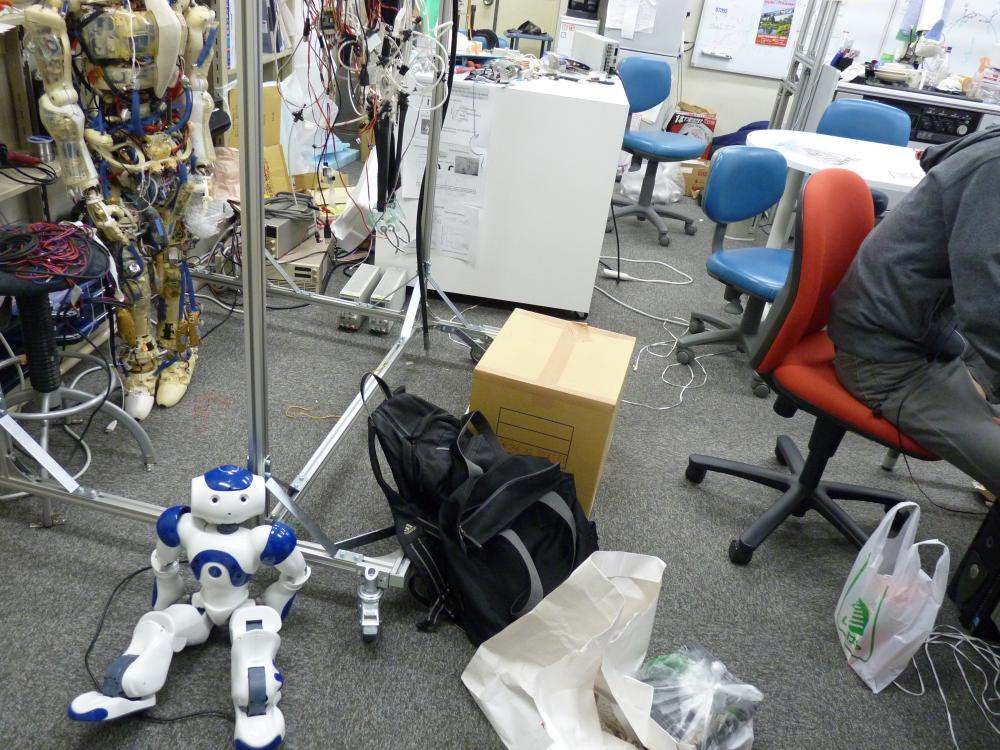
\includegraphics[width=0.50\hsize]{\FIGDIR/photo.jpg}%
    \caption{図の貼り方}%
    \label{fig:lab}%
  \end{center}%
\end{figure}%
図\ref{fig:lab}はこのようにして貼られた図である.
図に対して言及するときはこのようにrefコマンドを使う.
refコマンドの引数を,図を貼った時のコマンド群中のlabelコマンドの引数と対応させることで,意図した図に対してrefすることができるのである.

さて,先ほどの図の貼り方はちょっとめんどくさい.
大体,たかが図を一枚貼るためにこんな数行使った処理をいちいち書いてられないし,ソースコードのスペース的にもたくさん消費してしまってアホみたいである.
そのあたりを解決するのが,figコマンドである.
(figコマンドはいわば自作関数で,ikuo.styの中に定義されている.)
figコマンドを使うと,下記のように図を貼ることができる.
\fig{photo.jpg}{width=.50\hsize}{figコマンドを使って貼った図}
\figref{photo.jpg}はfigコマンドを使って貼った図である.
そして,今,気づいただろうか.
今のrefはただのrefではなく,figrefコマンドを使ってrefを行ったものである.
(figrefコマンドもfigコマンド同様にikuo.styの中で定義されている.)
figrefコマンドを使うと,いちいち「図」とか「fig.」とかをrefコマンドの前に書く必用がなくなり,便利である.
更に,「図」でなく「fig.」として参照するように変更する必用が生じた時にも,ikuo.styの中のfigrefコマンドの定義箇所にて変更をするだけで文書全体に変更が行われるのでとても有用であり,figrefコマンドを使わないのは愚かしい行為である.


\subsection{figに関連する便利コマンド}

figコマンドには残念ながら,図の位置を指定する引数が存在しない.
figコマンドの定義を見ると,位置指定オプションは[tbp]となっており,ページ上端,下端,まるまる1ページ,という優先度で位置が指定されることがわかる.
どうしてもページ下端に図を貼りたいんだ,という時にはfigbコマンドが用意されている.
\figb{photo2.jpg}{width=.50\hsize}{figbコマンドを使って貼った図}
\figref{photo2.jpg}はfigbコマンドを使って貼った図である.

どうしても位置を自分で指定したい,という場合はfigposコマンドを使う.
figposコマンドは第4引数が位置指定オプションに反映されるため,下記のように使うことができる.
\figpos{photo3.jpg}{width=.50\hsize}{figposコマンドを使って貼った図}{t}
\figref{photo3.jpg}はfigposコマンドを使って貼った図である.

上記各コマンドと合わせ,定義されているfig関連のコマンドを以下にまとめておく.
\begin{itemize}
\item fig\\
  図を貼るときに使う一番基本的なコマンド.
  位置指定は[tbp]となる.
  
\item twofigs\\
  2枚の図を立てに並べて貼るときに使うコマンド.
  キャプションは1つだけつき,ラベルは最初の図のファイル名になる.
  位置指定は[tbp]となる.
  
\item figthroug\\
  複数段組の文書中で,段組をぶちぬいて図を貼るときに使うコマンド.
  
\item figb\\
  ページ下端に図を貼るときに使うコマンド.
  
\item figpos\\
  任意の位置を指定して図を貼るときに使うコマンド.
  
\item doublefig\\
  2枚の図を横に並べて貼るときに使うコマンド.
  キャプションは1つだけつき,ラベルは最初の図のファイル名になる.
  位置指定は[tb]となる.
  
\item doublefigt\\
  doublefigコマンドと同様だが,ページ上端に図を貼るとき専用のコマンド.
  具体的には図の上側にスペースを入れずに貼ることができる.
  
\item doublefigb
  doublefigコマンドと同様だが,ページ下端に図を貼るとき専用のコマンド.
  
\item doublefigthrough\\
  doublefigコマンドと同様だが,複数段組の文章中で段組をぶちぬいて図を貼るときに使うコマンド.
  位置指定は[t]となる.
  
\item triplefig\\
  3枚の図を横に並べて貼るときに使うコマンド.
  キャプションは1つだけ表示され,ラベルは最初の図のファイル名になる.
  位置指定は[tbp]となる.
  
\item triplefigthrough\\
  triplefigコマンドと同様だが,複数段組の文章中で段組をぶちぬいて図を貼るときに使うコマンド.
  位置指定は[tbp]となる.
  
\end{itemize}


\section{表と式の書き方}
\seclabel{table_equation}

\subsection{表の書き方}
表を書くときには以下のようにする.
\begin{table}[tb]
  \label{sample}
  \begin{center}
    \caption{各人データ}
    \begin{tabular}{l|c|c|r}
      \hline
      名前 & 身長[cm] & 体重[kg] & 備考 \\
      \hline
      Y.M & 1800 & 60 & \\
      Y.M & 170 & 10 & \\
      Y.M & 170 & 60 & はげ\\
      \hline
    \end{tabular}
  \end{center}
\end{table}
表\ref{sample}は最も基本的な表の書き方の例である.
ソースコードを見ればわかる通り,この中ではlabelコマンドが使われているのだが,より便利なコマンドとしてtablabelが用意されている.
tablabelコマンドは表に対するラベルであるという情報をを自動的に付与してくれるため,これを用いることで図や式に対するラベルとごっちゃになるという問題を防ぐことができる.
同様のコマンドとしてfiglabel(図に対するラベル),equlabel(式に対するラベル),chaplabel(章に対するラベル),seclabel(節に対するラベル),subseclabel(小節に対するラベル)などが存在するので使うと良い.
\secref{fig}において用いたfigだとかtwofigだとかいった便利コマンドにおいてはその中でfiglabelが使用されている.

tablabelコマンドを用いた表は以下のようになる.
\begin{table}[tb]
  \tablabel{sample2}
  \begin{center}
    \caption{各人データ}
    \begin{tabular}{l|c|c|r}
      \hline
      名前 & 身長[cm] & 体重[kg] & 備考 \\
      \hline
      Y.M & 1800 & 60 & \\
      Y.M & 170 & 10 & \\
      Y.M & 170 & 60 & はげ\\
      \hline
    \end{tabular}
  \end{center}
\end{table}
\tabref{sample2}のようにtablabelを用いて表を書くと,tabrefコマンドを使うのが便利になる.
tabrefコマンドはfigrefコマンドのように自動で「図」とか「table」とかをつけてくれる便利コマンドである.

表に関しては特にこれ以上ローカルなコマンドとかないので,あとは研究室wikiを見るなりネットで情報探すなりして自分の書きたい表を書けるようになってください.


\subsection{式の書き方}
式は例えば以下のように書く.
\begin{eqnarray}
  \equlabel{hoge}
  hoge=hage
\end{eqnarray}

式に関してここで述べるべきことは表に関するそれとほぼ同様であり,つまりequlabelおよびequrefを使うべきであるという点のみである.
\equref{hoge}はequlabelを使ってラベル付されており,本文章冒頭のrefはequrefを用いて行われている.
式の書き方に関するそれ以外の情報は研究室wikiなりネット上で情報探すなりしてください.


\addcontentsline{toc}{chapter}{謝辞}
\markboth{謝辞}{謝辞}
% \chapter*{謝辞}
本論文は,筆者が東京農工大学大学院生物システム応用科学府生物機能システム科学専攻博士前期課程に在学中に行った研究をまとめたものです.\\
 本論文をまとめるにあたり,丁寧なご指導ご鞭撻を賜った東京農工大学生物システム応用科学府生物機能システム科学専攻 水内郁夫教授に深く感謝の意を表します.水内先生には貴重なご意見や適切なご指導をいただき,充実した研究生活を送ることができました.また,目上の方に対する礼儀はもちろん,研究報告会等私の今後の人生に重要な知識・経験をご教授していただく機会も多く,大変貴重な日々でした.改めて心より感謝申し上げます.\\
 森下克幸助教にも深く感謝の意を表します.森下先生には普段から積極的にコミュニケーションを取っていただき,その都度貴重なご意見をいただきました.お気遣いいただいたこともあり,研究をより充実したものにしていただきました.\\
 本学在籍時に関わった研究室のメンバーには大変お世話になりました.特に同期の長田京右さん,菅野公景さん,高橋龍乃介さん,山本雄大さんは共に過ごす時間も長く大変お世話になりました.長田くんとは研究活動外でも共に行動することが多く,他愛もない会話をしていつも楽しませてくれました.菅野くんは頼りになる研究時と研究外のギャップが大きく,いつも笑わせてくれました.高橋くんとは話すたびにふざけ合って,疲れを吹き飛ばしてくれました.山本君は研究テーマも近く,また夜中に研究室で話をしたりして切磋琢磨することができました.また,先輩の赤羽聖さんにも大変お世話になりました.研究時の研究外でも頼れる兄貴分的な存在であり,いつも支えていただきました.また,M1とB4の後輩たちにも大変お世話になりました.先輩後輩の垣根を越えて交流をしてくれたおかげで,研究生活が一層楽しいものになりました.これからもより一層頑張ってください.\\
 最後に,学費の援助,生活の支援をしてくれた両親に,心より感謝申し上げます.学生生活で多くの経験をすることができたのも両親による支えがあったからであると感じています.本当にありがとうございました.


\addcontentsline{toc}{chapter}{参考文献}
\markboth{参考文献}{参考文献}
\bibliographystyle{junsrt}
\bibliography{reference}

\end{document}
